\chapter{Empirical Data Analysis}
\label{ch:empirical-data-analysis}

This chapter showcases the analytical possibilities of the \tech{ln-history} platform. 
By using the \service{ln-history-database} and \service{ln-history-api}, 
we conduct novel analyses of the \gls{ln} and update existing findings from previous literature. 
All analytical scripts and raw data underlying this chapter are available as open-source code\footnote{\url{https://ln-history.info/analysis}}.
The analysis is divided into two scopes:

\begin{itemize}
    \item \textbf{Short-Term Metadata (\autoref{sec:metadata-analysis}):} 
        Focuses on the real-time operational behaviour of the network and the performance of the gossip protocol over a constrained collection window.

    \item \textbf{Long-Term Topology (\autoref{sec:historic-gossip-analysis}):} 
        Examines the macroscopic evolution of the network graph from its inception to the present day.
\end{itemize}

\subsection*{Scope and Methodology}

The first section (\autoref{sec:metadata-analysis}) is limited to the continuous collection window 
maintained by the two \tech{ln-history} collector nodes. 
This window starts on January 14, 2026, to March 3, 2026, during which the platform operated without major outages. 
Both nodes were deployed using the default \gls{cln} (\code{v25.09}) configuration, 
meaning they actively maintained connections to ten peers to receive gossip messages. 

By utilizing the metadata enriched during this period, we examine the total volume of messages 
and the degree of data overlap between the two distinct points in the topology (\autoref{fig:network-gossip-volume-and-overlap}). 
After that, we calculate the absolute propagation lag of the \gls{ln} (\autoref{fig:propagation-lag}) 
and the inter-collection lag between our two collector nodes (\autoref{fig:inter-collection-lag}). 
Finally, we analyse node connectivity behaviour by showing the distribution of peer session lengths (\autoref{fig:peer-session-distribution}) 
and testing for correlations between session duration and overall node capacity (\autoref{fig:peer-session-correlation}).


The second section (\autoref{sec:historic-gossip-analysis}) utilizes the batch-import 
capabilities of the platform to dive into the historical evolution of the \gls{ln} topology. 
We establish a baseline by showing the overall volume and distribution of historic gossip messages (\autoref{fig:gossip-messages-distribution}). 
Using the platform's snapshot functionality, we focus on payment channels, 
which build the routing backbone of the \gls{ln}. 
By examining the channel lifetime distribution (\autoref{fig:channel-lifetime-distribution}), 
we gain insights into the capital efficiency of the network. 
We also investigate whether the capacity of a channel influences correlates 
with the lifetime of a channel lifetime (\autoref{fig:channel-lifetime-correlation}). 
We finish off by acknowledging that the \gls{ln} is a distributed and not strictly decentralized network, 
we analyse its structural centralization over time. 
Building upon the methodology introduced by \citeauthor{zabka_short_2022}~\cite{zabka_short_2022}, 
we calculate the Gini coefficient based on the \gls{bc} for each historical snapshot (\autoref{fig:betweenness-centrality-gini}) 
and track the share of total \gls{bc} commanded by the top percentiles of routing nodes (\autoref{fig:betweenness-centrality-top-percentiles}).
We see that only a handful of nodes are very central in the \gls{ln} and visualize their
dominance over time in a heatmap, see \autoref{fig:top-nodes-heatmap}.


\section{Gossip Metadata Analysis}
\label{sec:metadata-analysis}

We introduced the gossip protocol in \autoref{sec:ln-gossip-protocol}, showing 
how storage efficient the topology information is. 
%AVG length of the raw_bytes column * number of messages in time frame * 0.8
We begin by exploring the collected gossip messages, shedding light into the volume
as well as completeness.
First we quantify the daily message volume and empirically measure the message propagation across the network. 
Theoretically, the \gls{ln} gossip protocol aims for global \textit{consensus}, 
meaning every node should eventually receive every broadcasted message.


\subsection{Network Gossip Volume and Lag}

We start by showing the number of gossip messages in the time frame to estimate the baseline network volume. 
To assess propagation consistency, we evaluate the intersection of messages received 
by our two independent collector nodes (referred to as \textit{Alice} and \textit{Bob}).

\subsubsection{Network Gossip Volume and Overlap}

Both collector nodes operate independently and 
append a local \code{seen\_at} timestamp as soon as they receive a gossip message. 
This gives three scenarios: 
A gossip message may be observed exclusively by Alice, exclusively by Bob, or (successfully) by both nodes.

\begin{figure}[htbp]
    \centering
    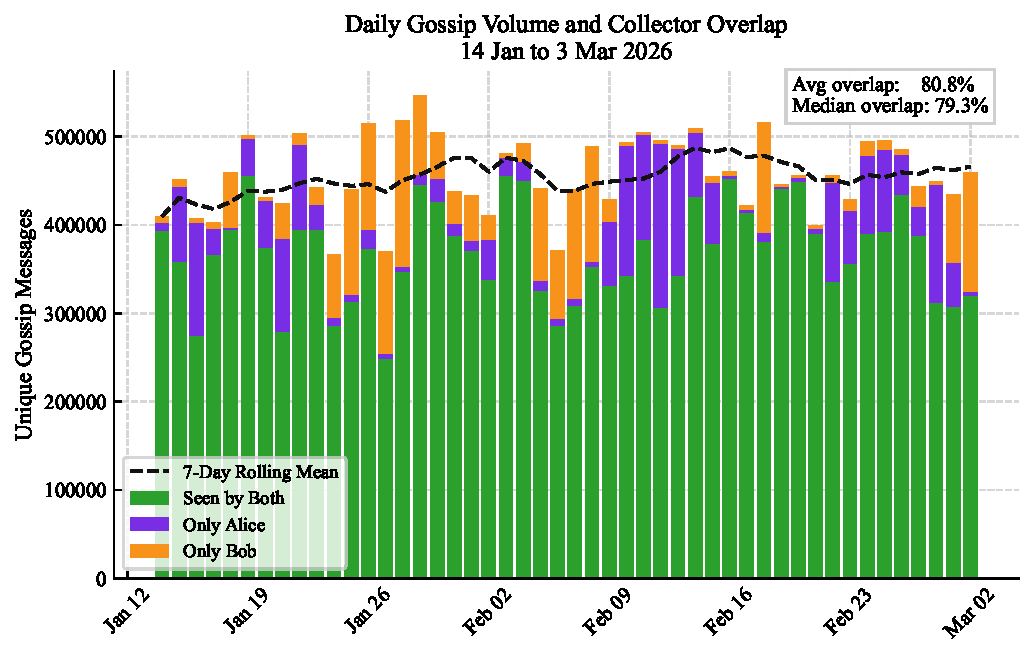
\includegraphics[width=0.7\linewidth]{resources/results-final/network-gossip-volume-and-overlap.pdf}
    \caption {
        In the measured time window around $400000$ unique messages have been seen by both nodes.
        The overall share of messages that have been received by both nodes is around $80\%$.
        Neither collector node has had an advantage sometimes Alice saw more, sometimes Bob. 
    }
    \label{fig:network-gossip-volume-and-overlap}
\end{figure}

The \autoref{fig:network-gossip-volume-and-overlap} shows that the rate of messages per day is rather constant
with a 7-day rolling average fluctuating between $400000$ and $500000$ unique messages.
The average overlap of $80.8 \%$ (median $79.3 \%$) shows that there are significant gaps in the gossip propagation.

We can also utilize the dataset to estimate the bandwidth requirements for operating a \gls{ln} node. 
\autoref{tab:message-footprint} presents the storage and message distribution grouped by type.

\begin{table}[htbp]
    \centering
    \caption{Storage footprint and message volume by gossip message type over the 48-day measurement window.}
    \begin{tabular}{@{} l r r r @{}}
        \toprule
        \textbf{Name} & \textbf{Avg Size (B)} & \textbf{Unique Msgs.} & \textbf{Total (MB)} \\
        \midrule
        Channel Announcement & 435.0 & \num{13045}     & 5.67    \\
        Node Announcement    & 502.3 & \num{6575334}  & 3302.95  \\
        Channel Update       & 143.0 & \num{14493905} & 2073.23  \\
        \bottomrule
    \end{tabular}
    \label{tab:message-footprint}
\end{table}

As \autoref{tab:message-footprint} shows, the total downloaded payload is \qty{4863}{\mega\byte} for Alice 
and \qty{4749}{\mega\byte} for Bob over the \num{48} consecutive days of measurement. 
This translates to a daily bandwidth requirement of roughly \qty{101.3}{\mega\byte} (\qty{98.9}{\mega\byte} respectively).
At the protocol level, this requires the node to process an average of \qty{4.6}{\text{messages}\per\second}. 
This demonstrates that the necessary bandwidth to run a \gls{ln} node, remains 
well within the constraints of standard consumer-grade internet connection.


\subsubsection{Propagation Lag}

When discussing protocol improvements it is useful to look at empirical measurements.
The propagation lag is calculated as the difference between the timestamp of the sender node $t_{sender}$
and the timestamp when a collector node has seen it $t_{seen}$: $|t_{seen} - t_{sender}|$.

In case both collector nodes have seen it at timestamp $t_{Alice}$ and $t_{Bob}$,
the first timestamp is chosen $t_{seen} = \min(t_{Alice}, t_{Bob})$. 

We group these measurements by message type, 
as each type serves a fundamentally different operational role within the network.

\begin{figure}[htbp]
    \centering
    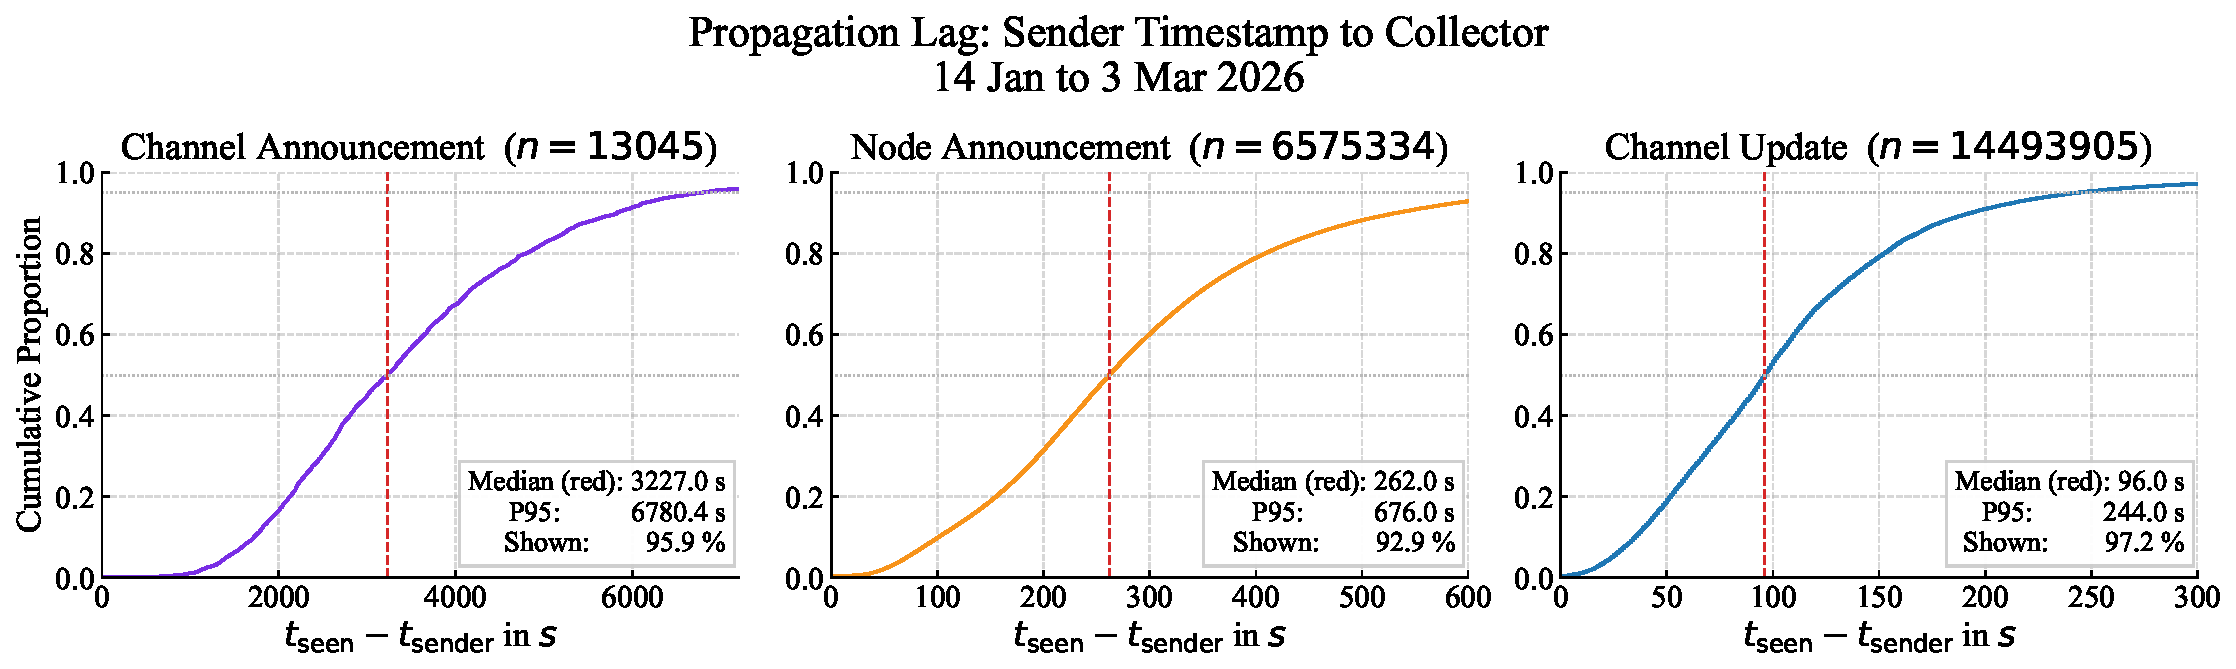
\includegraphics[width=\textwidth]{resources/results-final/propagation-lag-large.pdf}
    \caption{
        The Lag between the message type differs enormously depending on the message type.
        \code{Channel\_announcements} take on median around \qty{3227}{\second} and are an order of magnitude 
        slower than \code{node\_annoncements} and \code{channel\_updates} which respectively 
        only have (on median) \qty{262}{\second} and \qty{96}{\second}.
    }
    \label{fig:propagation-lag}
\end{figure}

\autoref{fig:propagation-lag} illustrates the propagation lag in a \gls{cdf} chart grouped my messages type.
\code{Channel\_announcement} propagation is much slower with \qty{3227}{\second} 
(approximately \num{54} minutes) due to the on-chain footprint.
As mandated by the BOLT specification, nodes must wait for six block confirmations
before broadcasting the announcement to the public network~\cite{lightningdevelopers_bolts_2018}. 
This mandatory waiting period artificially inflates the measured propagation lag.

It is also notably to see how steep the curves grow.
As \code{node\_announcements} are in most cases heartbeats with redundant information 
it is less urgent for them to spread quickly resulting in a lag of \qty{262}{\second} (more than \num{4} minutes).
But as \code{channel\_updates} play an important role in routing payments, their information spreading is urgent
achieving a median lag of only \qty{96}{\second}.


\subsubsection{Inter Collection Lag Distribution}
While absolute propagation lag measures the delay from the origin, 
the \term{inter-collection lag} evaluates the synchronization between the two independent
positions of \textit{Alice} and \textit{Bob} in the \gls{ln}. 

It is defined as the absolute difference between the collection timestamps of Alice and Bob
for a given unique message: $|t_{Bob} - t_{Alice}|$. 

This metric could answer whether two distinct, standardly configured \gls{cln} nodes receive 
the same network updates concurrently or if there is a significant synchronization delay between different network clusters.

\begin{figure}[htbp]
    \centering
    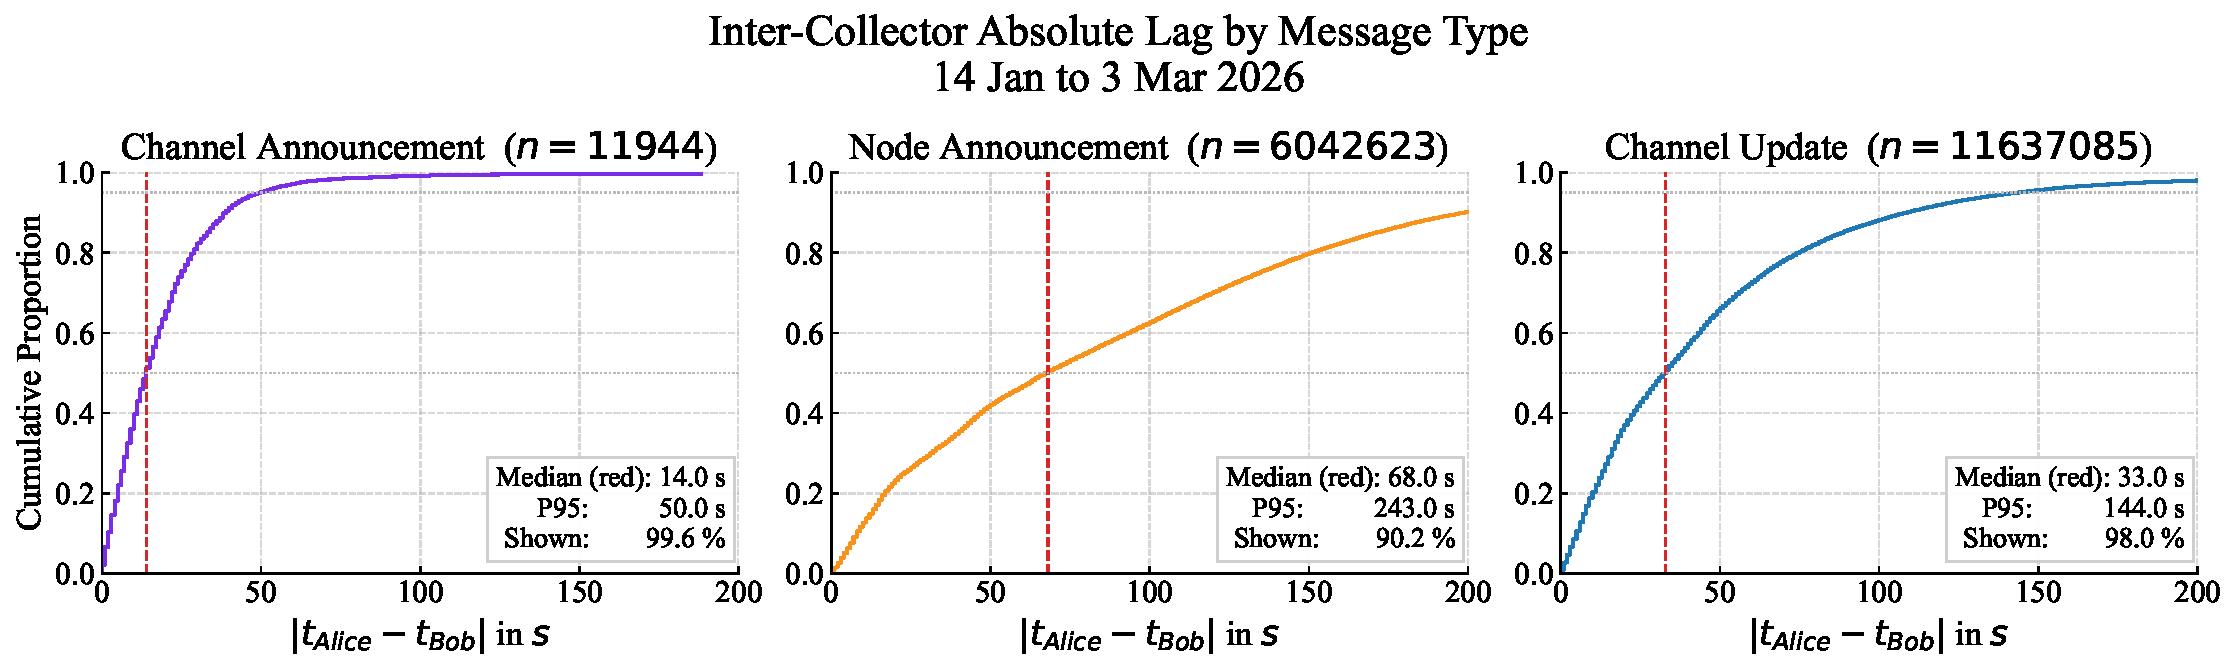
\includegraphics[width=\textwidth]{resources/results-final/inter-collector-lag-large.pdf}
    \caption{
        Distribution of the absolute inter-collection lag between the two collector nodes, 
        categorized by gossip message type.
        Two \gls{cln} nodes with the default configuration recieved 
        \code{channel\_announcements} closely with only \qty{14}{\second} difference.
        Further \code{node\_announcement} messages on median have a bigger variation of over a minute (\qty{68}{\second}).
        \code{Channel\_updates} lay in between with an absolute difference of \qty{33}{\second}
        The resolution is scaled to one second.
    }
    \label{fig:inter-collection-lag}
\end{figure}

To ensure the integrity of the measurement, extreme anomalies caused by a collector crash
were removed to isolate the steady-state network behaviour. 
The resulting distribution is shown in \autoref{fig:inter-collection-lag}.

An interesting observation is the steepness with which the \gls{cdf} curves drop, 
highlighting a generally high degree of synchronization between the two collector nodes. 
However, the exact synchronization speed varies significantly depending on the message type.

The \code{node\_announcements} on the other hand get received at much different times.
As they do not have an immediate effect on payment routing, this is not worrying.

Every channel must have at least one \code{channel\_update} message referenced to it,
so that the routing policy are met during payment routing.
The fact that it takes only $33 s$ on median per \code{channel\_udpate} message,
shows that they propagate much quicker.

\code{Channel\_announcement} messages are synchronized tightly, 
with a median inter-collection lag of only \qty{14}{\second}. 
Furthermore, the \num{95}th percentile is reached at just \qty{50}{\second}. 
This indicates that once a new channel is propagated the parallel network paths ensure 
both nodes discover it almost simultaneously.

Similarly, \code{channel\_update} messages are synchronized quickly, 
with a median absolute difference of \qty{33}{\second}. 
Because every active channel must maintain the latest routing policies to successfully route payments, 
the \gls{ln} focuses on rapid synchronization of these updates. 

On the other hand, \code{node\_announcement} messages exhibit a much wider variance, 
with a median lag of \qty{68}{\second}. 
Because these messages function primarily as informational heartbeats and do not have an immediate impact on payment routing, 
they are not as prioritized as the other two message types.


\subsection{Peer Session Analysis}
\label{sec:peer-session}

Empirical research regarding the long-term peer management behaviour of Lightning Network nodes (specifically \gls{cln} implementation) is rare.
Because the gossip protocol relies on active \gls{p2p} connections to propagate messages, understanding the connection stability is important. 
Utilizing the \service{peer-manager} component, the \tech{ln-history} platform continuously logged the lifecycle of all peer sessions established by 
our two collector nodes (\textit{Alice} and \textit{Bob}).

In this section we first show the distribution of peer session durations.
Next, we investigate whether a correlation exists between a peer's node size and its connection stability.

\subsubsection{Peer Session Distribution}
For the \gls{ln} to work, it is necessary that nodes receive gossip messages, but
there is no enforcement for nodes to send it.
As the collector nodes do not maintain any channels, some peers do not see a reason
to share their gossip to them, since they do not need it as they cannot route payments.

\begin{figure}[htbp]
    \centering
    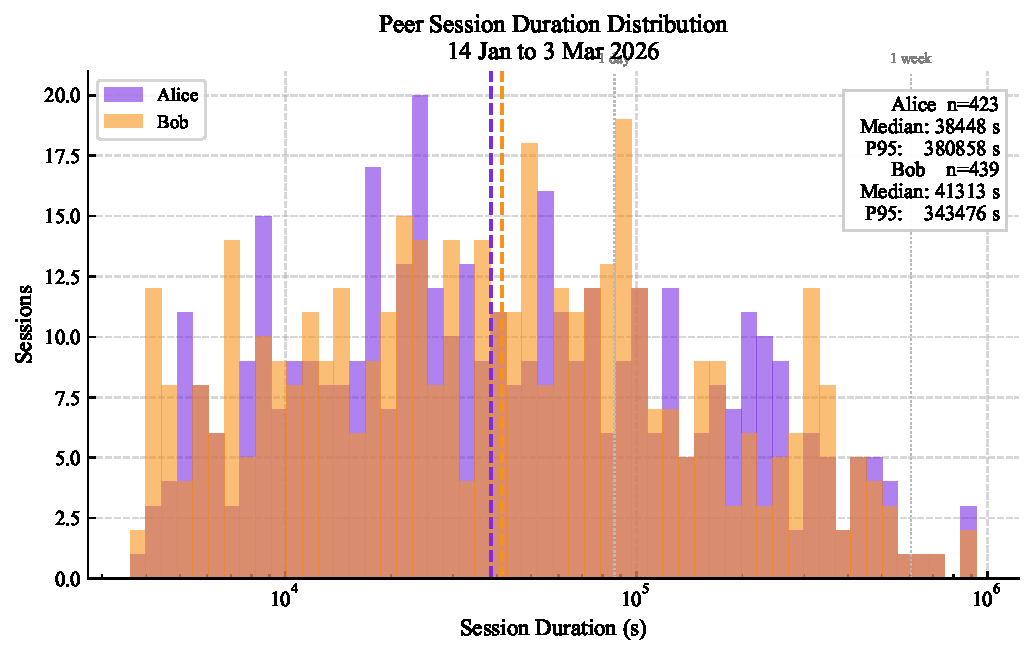
\includegraphics[width=0.7\textwidth]{resources/results-final/peer-session-distribution.pdf}
    \caption{
        Distribution of peer sessions with the collector nodes (\textit{Alice} and \textit{Bob}) 
        show that they have roughly the same number of connections ($423$ and $439$) in the time frame.
        The session durations vary a lot but have approximately the same median at around 11 hours.
    }
    \label{fig:peer-session-distribution}
\end{figure}

The \autoref{fig:peer-session-distribution} shows that the duration of peer
sessions varies between $30 min$ to up to over a week with a median at
$10.7 h$, $11.5 h$ for respectively \textit{Alice}, \textit{Bob}.


\subsubsection{Correlation between Peer Session Duration and Node Size}
Depending on the operational goals of a \gls{ln} node, 
actively selecting reliable peers for gossip propagation is advantageous. 

A sustained, uninterrupted \gls{p2p} connection implicitly indicates that the peer possesses 
a stable internet connection and robust underlying hardware. 

Therefore, we use the session duration as a proxy metric for the infrastructure reliability of the peer node.

\begin{figure}[htbp]
    \centering
    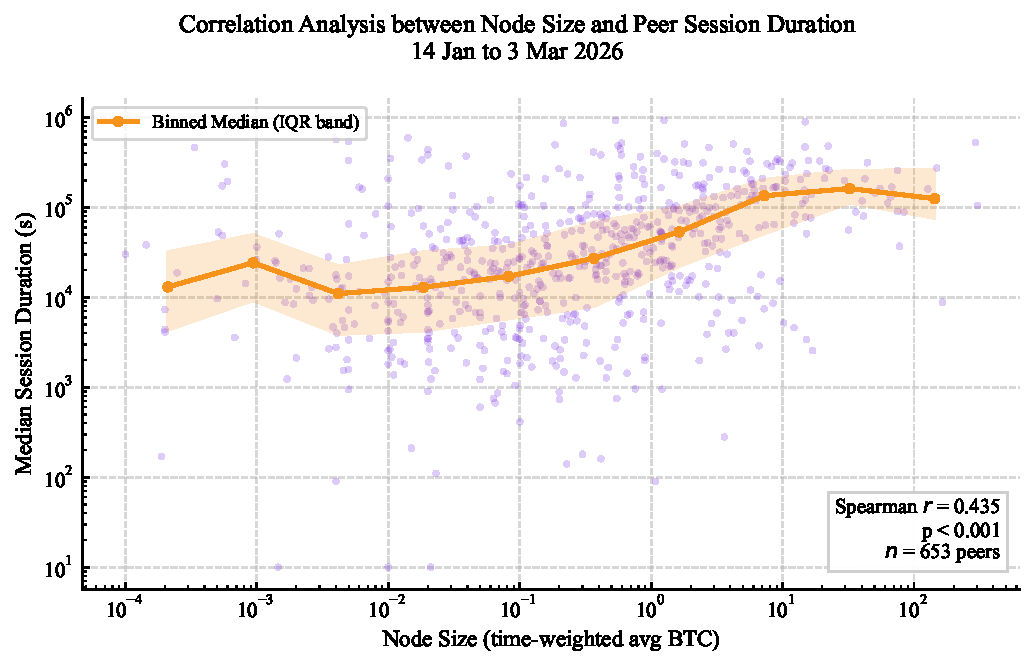
\includegraphics[width=0.7\textwidth]{resources/results-final/corelation-node-size-and-session-duration.pdf}
    \caption{
        A trend exists that larger nodes tend to support longer sessions with a 
        correlation coefficient $r = 0.435$ (statistical significance $p < 0.001$).
        The node sizes indicated as purple dots are binned into \num{10} bins. t
        The orange dots represent their median and the area around the graph shows 
        the 25th and 75th percentile of each bin.
    }
    \label{fig:peer-session-correlation}
\end{figure}

The \autoref{fig:peer-session-correlation} shows a moderate but positive correlation 
(Pearson's $r = 0.435$, $p < 0.001$) between the node size and the session duration. 
This trend suggests that highly capitalized routing nodes are generally operated 
on professional (high-availability) infrastructure, leading to fewer connection drops.

For node operators, this finding offers a strategy to mitigate the gossip synchronization blind spots
which were shown in \autoref{fig:network-gossip-volume-and-overlap}.
\\


\section{Historic Gossip Analysis}
\label{sec:historic-gossip-analysis}

This section analyses the complete set of public gossip messages collected between 2018 and April 2026
and persisted in the \tech{ln-history} platform, which in total are approximately \num{91.3} million.


\subsection{Gossip Distribution}

To establish a foundational understanding of the dataset, we first examine the historic distribution of gossip messages categorized by their respective types. 
After that, we utilize the \service{ln-history-api} to generate snapshots of the network graph, allowing us to analyse topology changes over time.
 
As defined in the BOLT specifications, \code{node\_announcement} and \code{channel\_update} messages have a \code{timestamp} field. 
Because \code{channel\_announcement} messages lack this field, we utilize the \code{funding\_timestamp} 
which is the confirmation time of the underlying funding transaction. 
Aggregating these timestamps allows us to visualize the monthly volume of the entire dataset.


\begin{figure}[H]
    \centering
    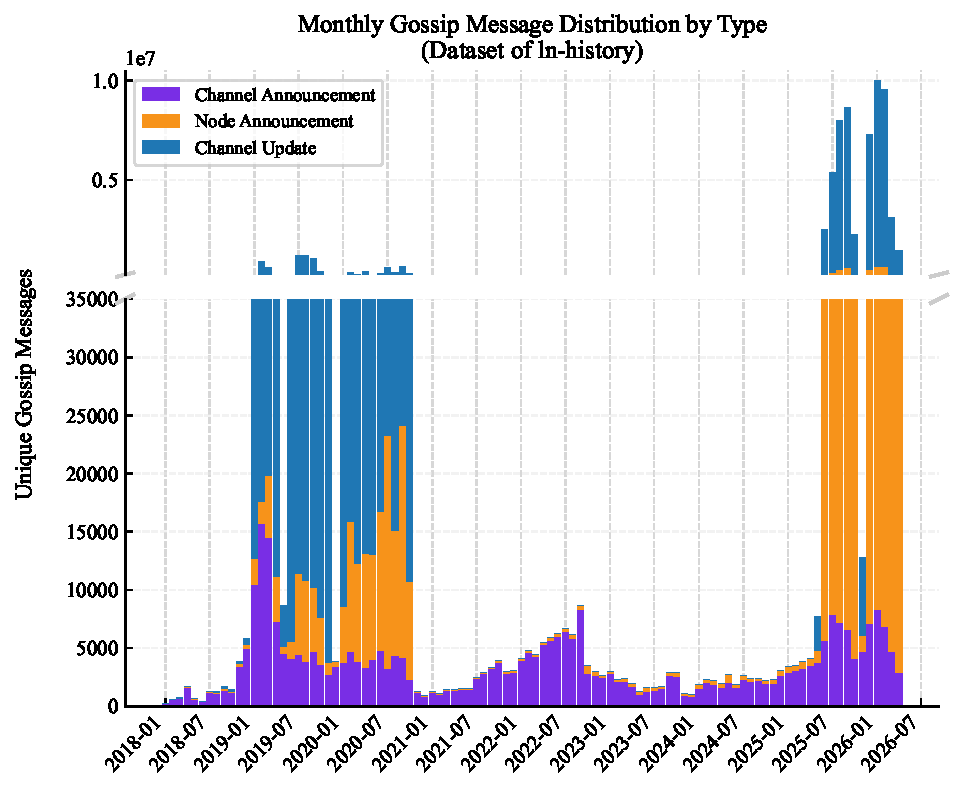
\includegraphics[width=0.7\textwidth]{resources/results-final/gossip-distribution-by-type.pdf}
    \caption{
        Monthly distribution of collected gossip messages by type. 
        The timeline highlights two distinct periods of intensive data archiving: 
        The initial 2019-2021 dataset provided by \citeauthor{decker_lnresearch_2020}~\cite{decker_lnresearch_2020}, 
        and the ongoing \tech{ln-history} collection beginning in mid-2025. 
    }
    \label{fig:gossip-messages-distribution}
\end{figure}

\autoref{fig:gossip-messages-distribution} provides insight into both the composition of the gossip messages and the share of the preserved data. 
Under active monitoring conditions, \code{channel\_updates} constitute the vast majority of all broadcasted messages, 
followed by \code{node\_announcements}, while structural \code{channel\_announcements} 
represent the smallest fraction of total traffic. 

Furthermore, the timeline illustrates two distinct periods of intensive data collection. 
The initial continuous block (from 2019 to roughly 2021) represents the invaluable open-source dataset 
aggregated by \citeauthor{decker_lnresearch_2020}~\cite{decker_lnresearch_2020}. 
Unfortunately, active support for that specific public archive ceased and 
the dataset exhibits a gap where mainly structural \code{channel\_announcements} were reliably preserved.

The second spike of data represents the active operation of the \tech{ln-history} platform, 
which successfully bridges this historical data gap and ensures continuous, future-proof data collection. 

Beyond the collection mechanics, the data shows a trend that the overall volume of gossip 
network traffic has increased significantly as the \gls{ln} has grown.


\subsection{Channels}

Payment channels are the foundational scaling mechanism of the \gls{ln}. 
In this section, we analyse the operational lifetime of these channels and investigate 
whether a correlation exists between a channel's lifetime and its committed capacity.

\subsubsection{Distribution of Channel Lifetime}

The lifespan of a channel is limited by two on-chain events: 
its creation via a funding transaction, and its termination when the underlying funding \gls{utxo} is 
spent\footnote{Recent protocol advancements, such as \term{channel splicing}, allow a funding \gls{utxo} 
to be spent to resize a channel's capacity without disrupting its operational continuity from the user's perspective. 
However, for the historical topological analysis, any on-chain spending of the original funding \gls{utxo} is considered as a channel closure.}. 
By measuring the time difference between these two block timestamps, we can calculate the lifetime of every closed channel in our dataset.

\begin{figure}[htbp]
    \centering
    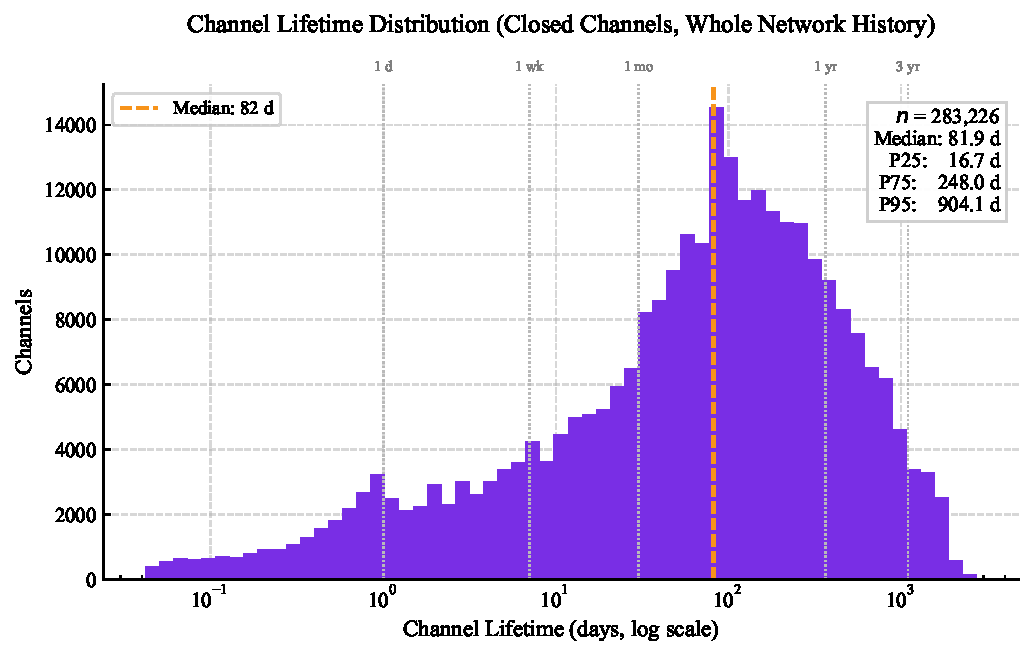
\includegraphics[width=0.7\textwidth]{resources/results-final/channel-lifetime-distribution.pdf}
    \caption{
        The median channel lifetime distribution of closed channels is \qty{105.6}{\day} days with a large variance.
        Some channels only exist for a few days whereas others survived multiple years. 
    }
    \label{fig:channel-lifetime-distribution}
\end{figure}


As shown in \autoref{fig:channel-lifetime-distribution}, the lifespan of \gls{ln} channels has a large variance. 
The median channel lifetime is \qty{81.9}{\day} (approximately three and a half months). 


On the one hand the distribution's long tail proves that stable channels surviving for multiple years do exist, 
but on the other hand the empirical data reveals a different reality for the majority of the network.

A significant concentration of channels exists at the extreme lower bound of the distribution, 
indicating that a substantial portion of channels are closed within just a few days of their creation.

It is important to note that this specific metric suffers from \textit{survivorship bias}. 
The calculation exclusively evaluates closed channels and therefore systematically excludes the network's 
long-living active channels that remain operational as of writing. 
We can therefore say that the true median lifetime of all successfully established \gls{ln} channels is likely
higher than what this subset suggests.


\subsubsection{Correlation between Channel Size and Channel Lifetime}

Because opening and closing channels costs on-chain Bitcoin mining fees, 
it is economically advantageous for node operators to maintain open channels for as long as possible. 
As established in \autoref{sec:peer-session}, well-capitalized node operators tend to have better infrastructure, 
resulting in higher reliability and longer peer sessions. 

A natural extension of this observation is to guess whether this operational professionalism translates to channel management. 
We investigate whether channels with higher capacity exhibit longer operational 
lifespans than smaller, potentially hobbyist-run channels.

\begin{figure}[htbp]
    \centering
    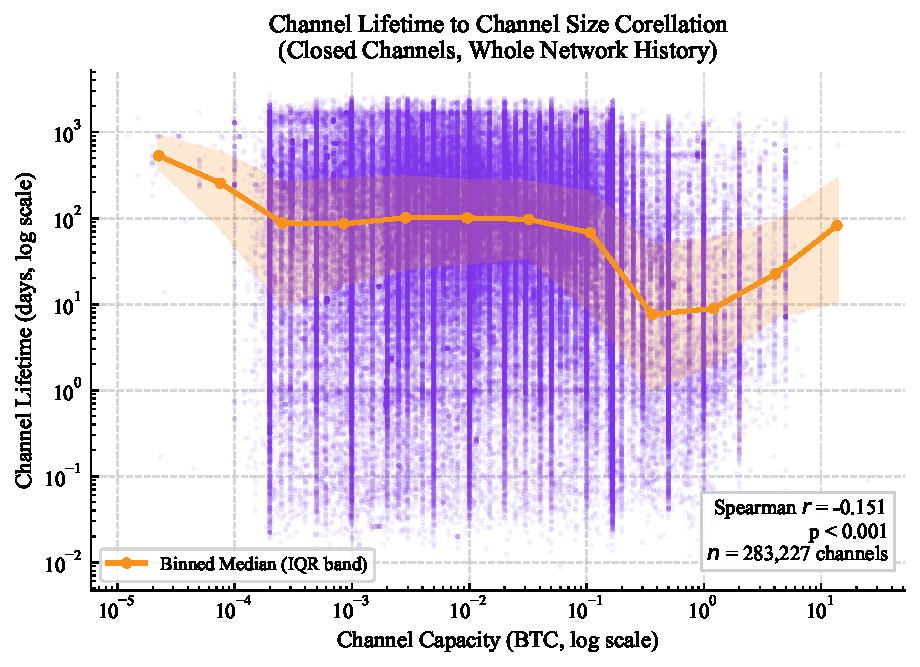
\includegraphics[width=0.7\textwidth]{resources/results-final/channel-capacity-lifetime-correlation.pdf}
    \caption{
        Scatter plot evaluating the relationship between a channel's capacity and its operational lifetime. 
        The data indicates no statistically significant correlation between the two variables.
    }
    \label{fig:channel-lifetime-correlation}
\end{figure}

Surprisingly, as illustrated in \autoref{fig:channel-lifetime-correlation}, 
the empirical data reveals absolutely no correlation between the channel capacity and its lifetime. 
It appears that channels are opened and closed at similar frequencies entirely independent of their capacity. 

This behaviour is likely compounded by the conditions of the Bitcoin mining fees. 
For the vast majority of the analysed timeframe, on-chain transaction fees remained low. 
When base-layer settlement costs are negligible, the financial penalty for closing and reopening channels is reduced, 
Therefore, closures are more likely dictated by other factors, like liquidity imbalances or active capital reallocation, 
which affect channels of all sizes.



\subsection{Centrality}
\label{sec:centrality}

This final section of the analysis chapter showcases how the snapshot generation 
of the \service{ln-history-api} can be used for in depth analysis of the topology of the \gls{ln}.

While graph centrality can be evaluated using a variety of metrics,
the main function of the \gls{ln} is payment routing.
The payment routing algorithms implemented by Lightning node clients use 
variations of Dijkstra's shortest-path algorithm~\cite{saraswathi_exposition_2024}.
This led to the selection of \gls{bc}. 
As defined by \citeauthor{newman2018networks}~\cite{newman2018networks}, 
\gls{bc} ranks each node based on the exact frequency of its occurrence along 
the shortest paths calculated between all possible node pairs in the network.


\subsubsection{Betweenness Centrality Concentration (Gini Coefficient)}

The Gini coefficient is a standard statistical metric used to quantify inequality within a distribution.
It is a number between \num{0} (perfect equality) and \num{1} (maximal inequality)~\cite{gini_variabilita_1912}. 

Applying the Gini coefficient to \gls{bc} to evaluate \gls{ln} centralization was first 
done by \citeauthor{zabka_short_2022} in \citetitle{zabka_short_2022}~\cite{zabka_short_2022}. 

In this section, we expand upon their foundational research. 
By utilizing the highly optimized snapshot creation of the \tech{ln-history} platform, 
we are able to compute these complex centrality metrics across a significantly higher temporal resolution 
and over a substantially extended historical time horizon.

\begin{figure}[htbp]
    \centering
    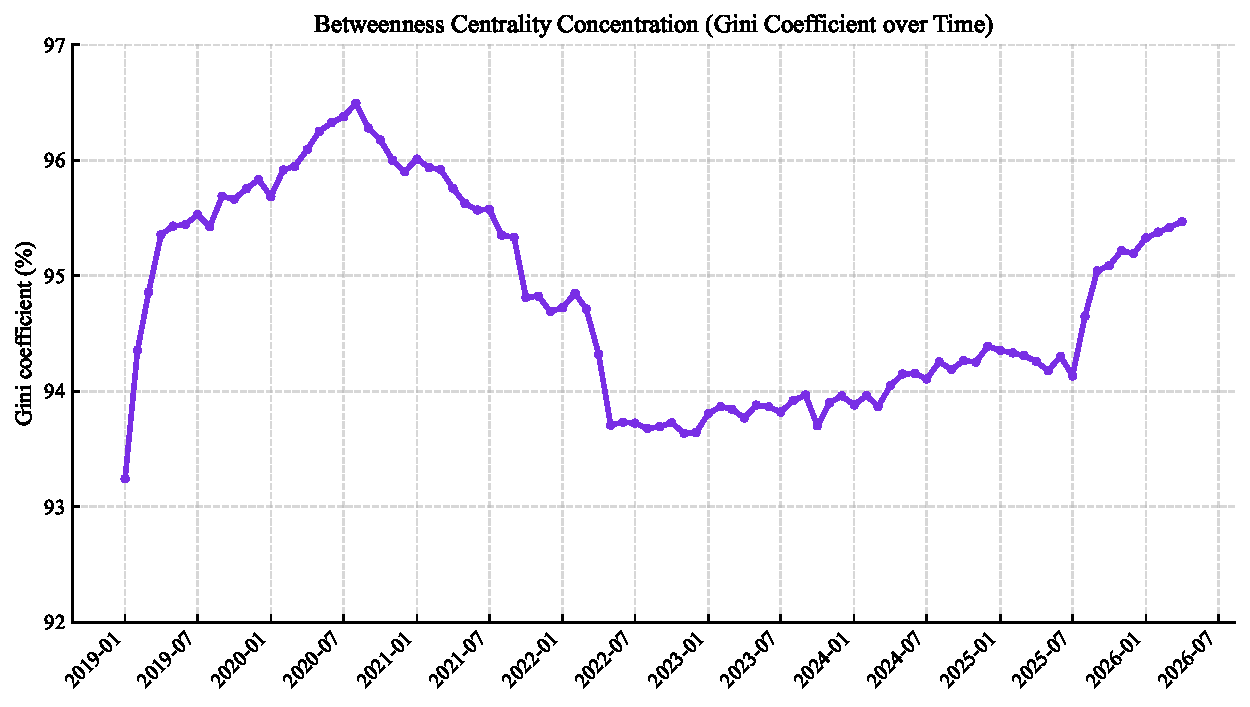
\includegraphics[width=\textwidth]{resources/results-final/centrality-gini.pdf}
    \caption{
        Gini coefficient of the \gls{bc} across network snapshots from 2018 to 2016, 
        With values abolve \qty{90}{\percent} the centrality of the \gls{ln} is high and has remained high.
    }
    \label{fig:betweenness-centrality-gini}
\end{figure}

As illustrated in \autoref{fig:betweenness-centrality-gini}, the Gini coefficient has remained high
with fluctuating values between \qty{93}{\percent} and \qty{97}{\percent}.

This result shows that almost every two pair of nodes when connected with the shortest path,
needs to route through the same few central nodes.

The implications of this topology will be discussed in the \autoref{ch:conclusion}.


\subsubsection{Betweenness Concentration by Top Percentiles over Time}
To further investigate this structural inequality, we categorize the routing nodes 
into percentiles based on their proportional share of the total network \gls{bc} over time.
\begin{figure}[htbp]
    \centering
    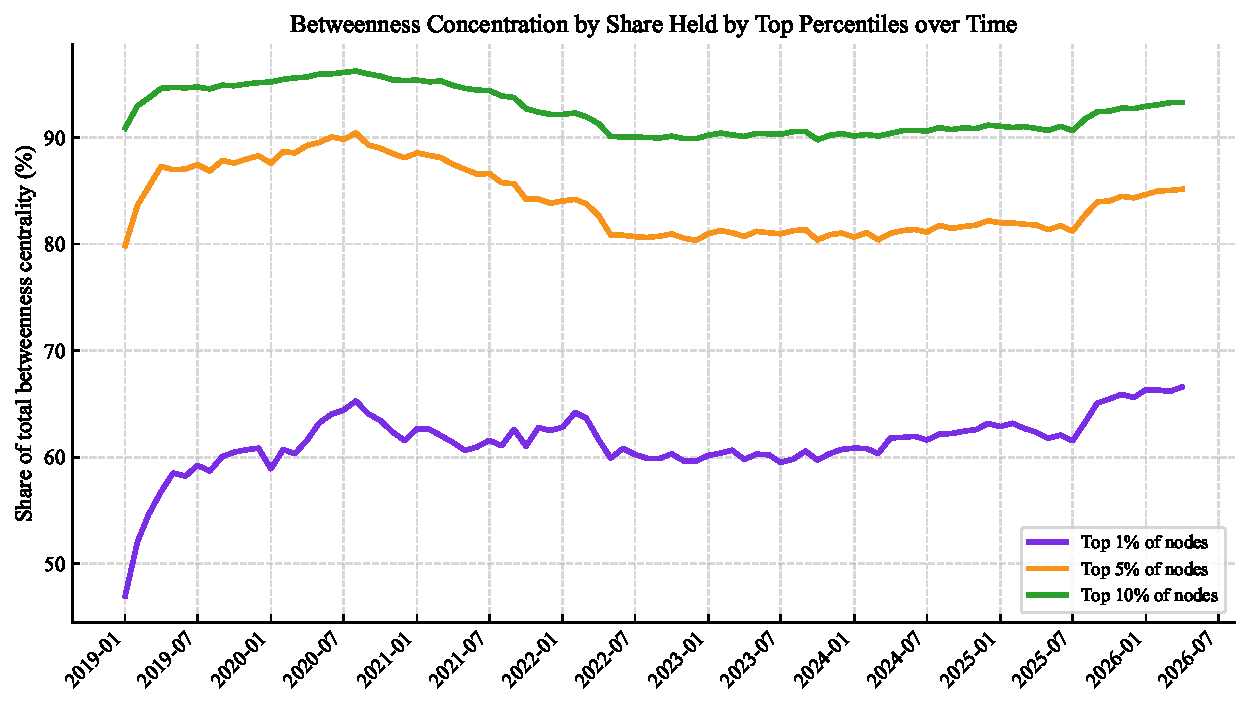
\includegraphics[width=\textwidth]{resources/results-final/centrality-concentration-top-percentiles.pdf}
    \caption{
        Since the beginning of the \gls{ln} the top \qty{1}{\percent} of nodes
        own more than \qty{50}{\percent} of the share of total \gls{bc}.
        Further, the top \qty{10}{\percent} around \qty{90}{\percent}.
    }
    \label{fig:betweenness-centrality-top-percentiles}
\end{figure}

The \autoref{fig:betweenness-centrality-top-percentiles} underlines the previous analysis 
that the \gls{ln} is centralized with only a few nodes having an enormous share of total \gls{bc}.
The top $10 \%$ of nodes posses over $90 \%$ of the total \gls{bc}.


\iffalse
\subsubsection{Lorenz Curve Evolution}
\begin{figure}[htbp]
    \centering
    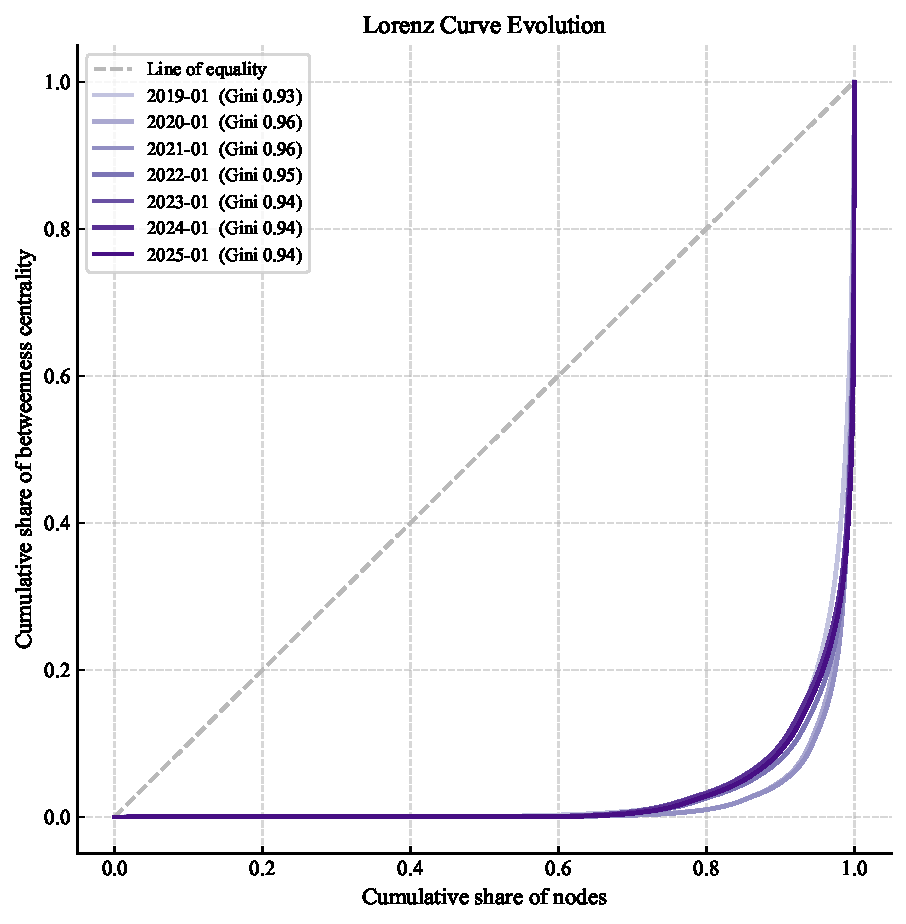
\includegraphics[width=\textwidth]{resources/results-final/lorenz-curve.pdf}
    \caption{
        Lorenz Cureve
    }
    \label{fig:lorenz-curve}
\end{figure}
\fi


\subsubsection{Heatmap of Top Nodes by Betweenness Centrality over Time}

To conclude this topological analysis, we determine the \gls{ln} most influential routing hubs.

We can name the exact nodes that have major influence in the \gls{ln}.
Over its lifetime of the \gls{ln} they have established themselves as important hubs.

By tracking the \gls{bc} rankings of individual nodes across the historical snapshots, 
we visualize the network's central hubs in a heatmap.

\begin{figure}[htbp]
    \centering
    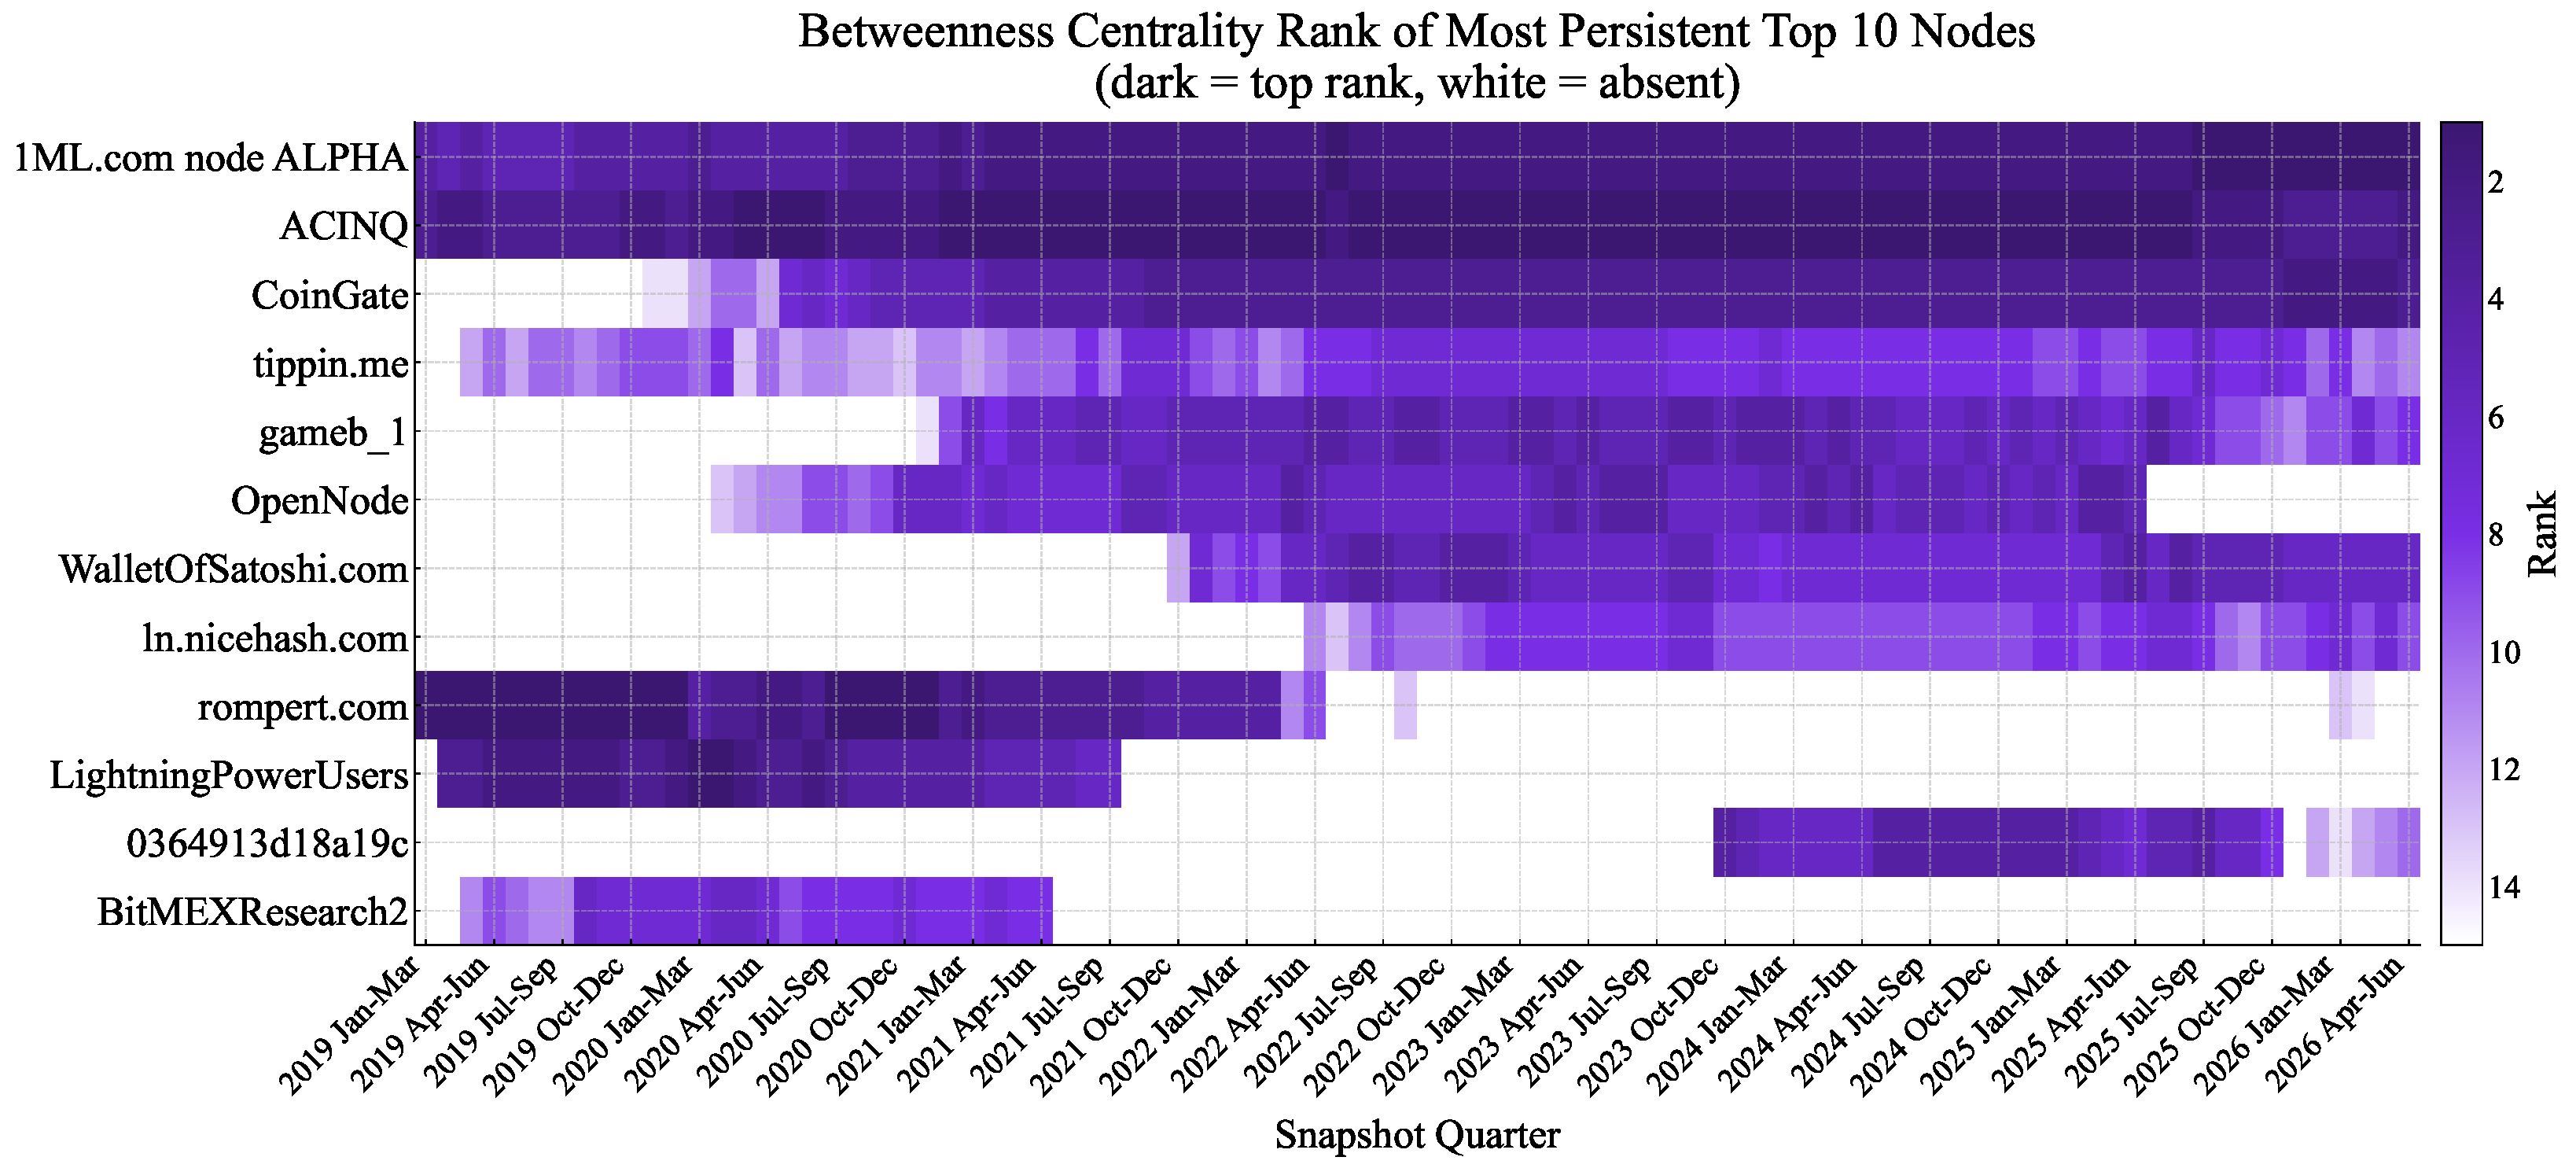
\includegraphics[width=\textwidth]{resources/results-final/centrality-top-nodes-heatmap.pdf}
    \caption{
        Heatmap tracking the betweenness centrality rankings of the most 
        central nodes across the whole history of the \gls{ln}.
    }
    \label{fig:top-nodes-heatmap}
\end{figure}

The \autoref{fig:top-nodes-heatmap} visualizes how a few nodes namely 
\textit{ACINQ}, \textit{1ML} and \textit{CoinGate} have dominated and still dominate
the network when looking at betweenness centrality ranking of the \gls{ln}.

We discuss the consequences of this in \autoref{ch:conclusion}.

\iffalse
Future ideas:

\item 4B Tor vs clearnet share of nodes per snapshot for every quarter of existing gossip

SUB Gossip analysis: which nodes send which gossip (redundant or actualy new information)
\item 1D Bigger nodes update more frequently, correlation?
\item 1E Bigger channels update more frequently?
\item 1F Looking at a channel: Does the bigger or smaller node update the fees more often?

\item 1G Distribution how many channel_update messages are actually new and which are redundant
\item 1H Divide the network into active and passive nodes based on channel_update msg
\fi